\section{Low Class Reference}
\label{classLow}\index{Low@{Low}}
{\tt \#include $<$low.h$>$}

Inheritance diagram for Low:\begin{figure}[H]
\begin{center}
\leavevmode
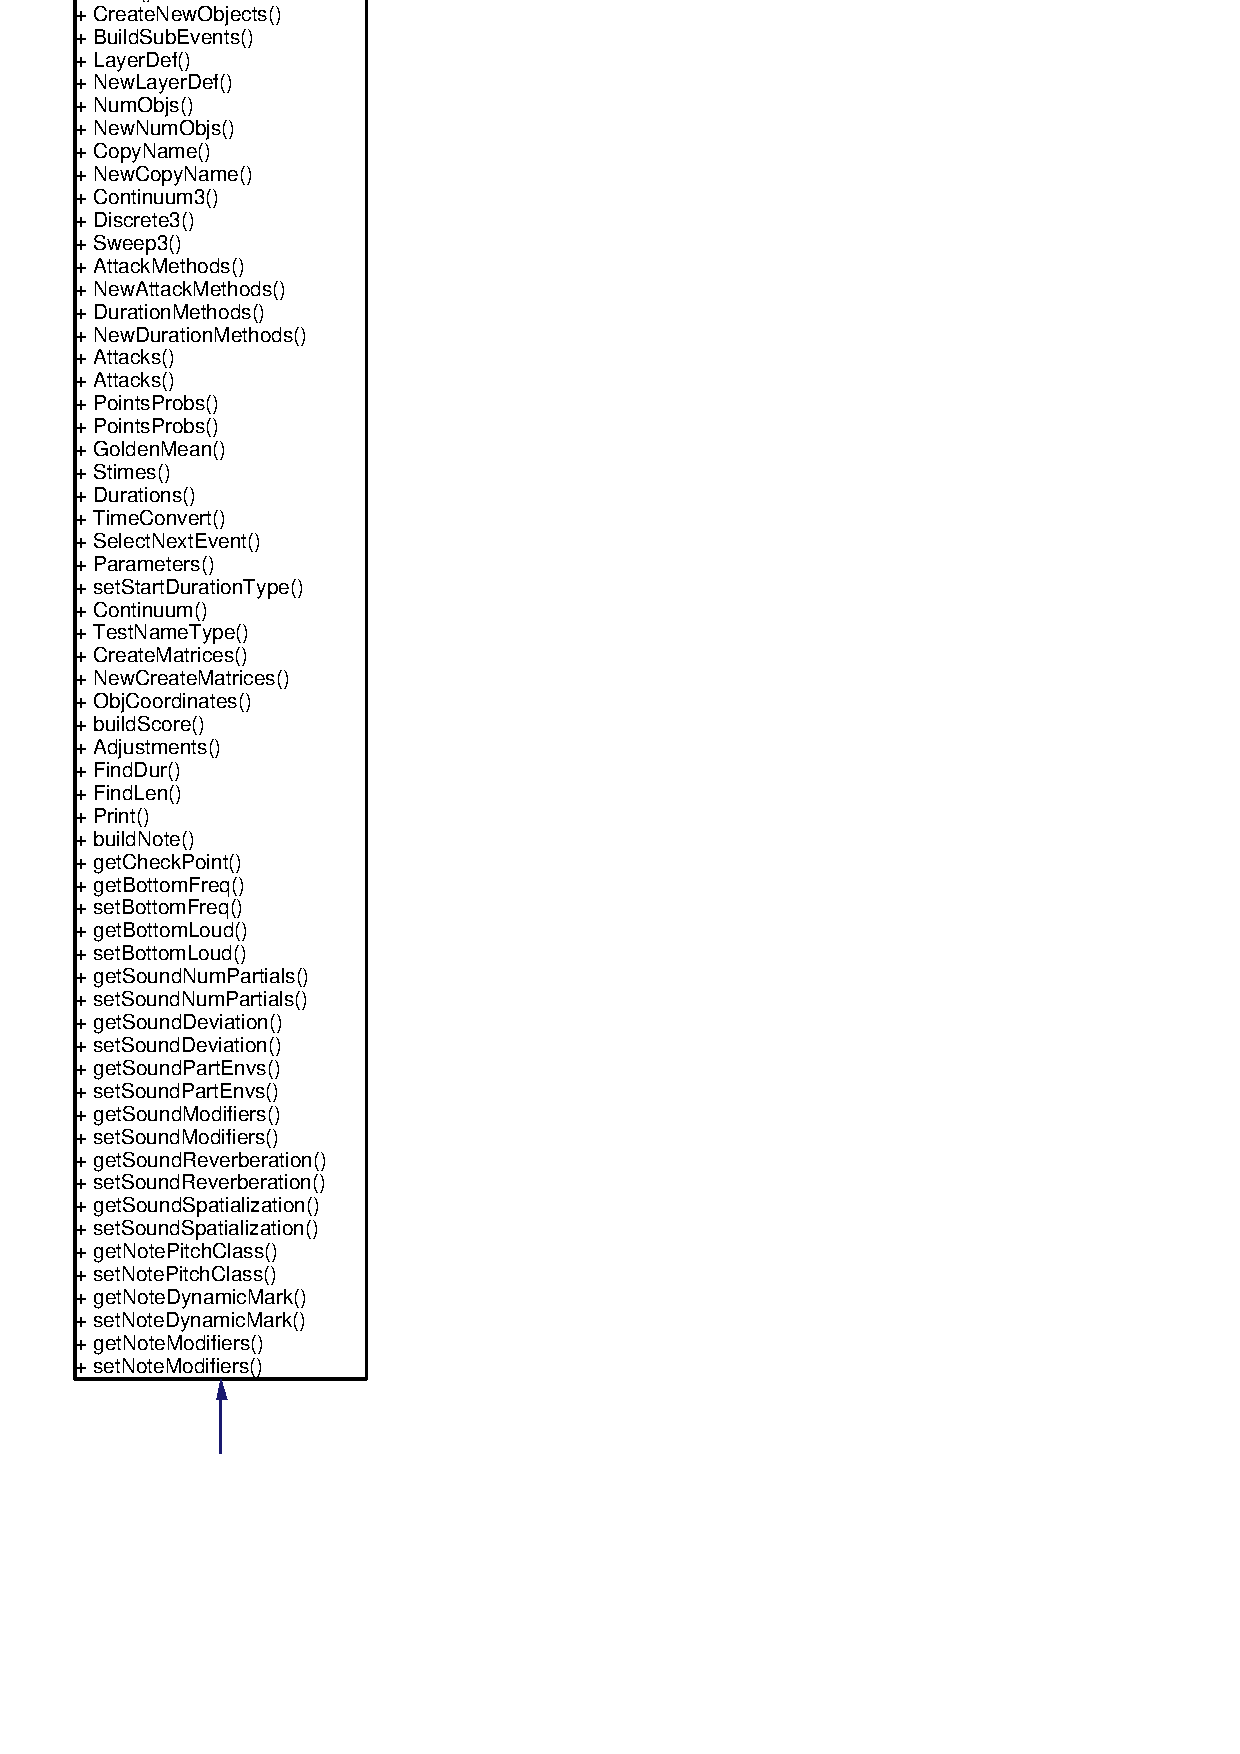
\includegraphics[width=88pt]{classLow__inherit__graph}
\end{center}
\end{figure}
Collaboration diagram for Low:\begin{figure}[H]
\begin{center}
\leavevmode
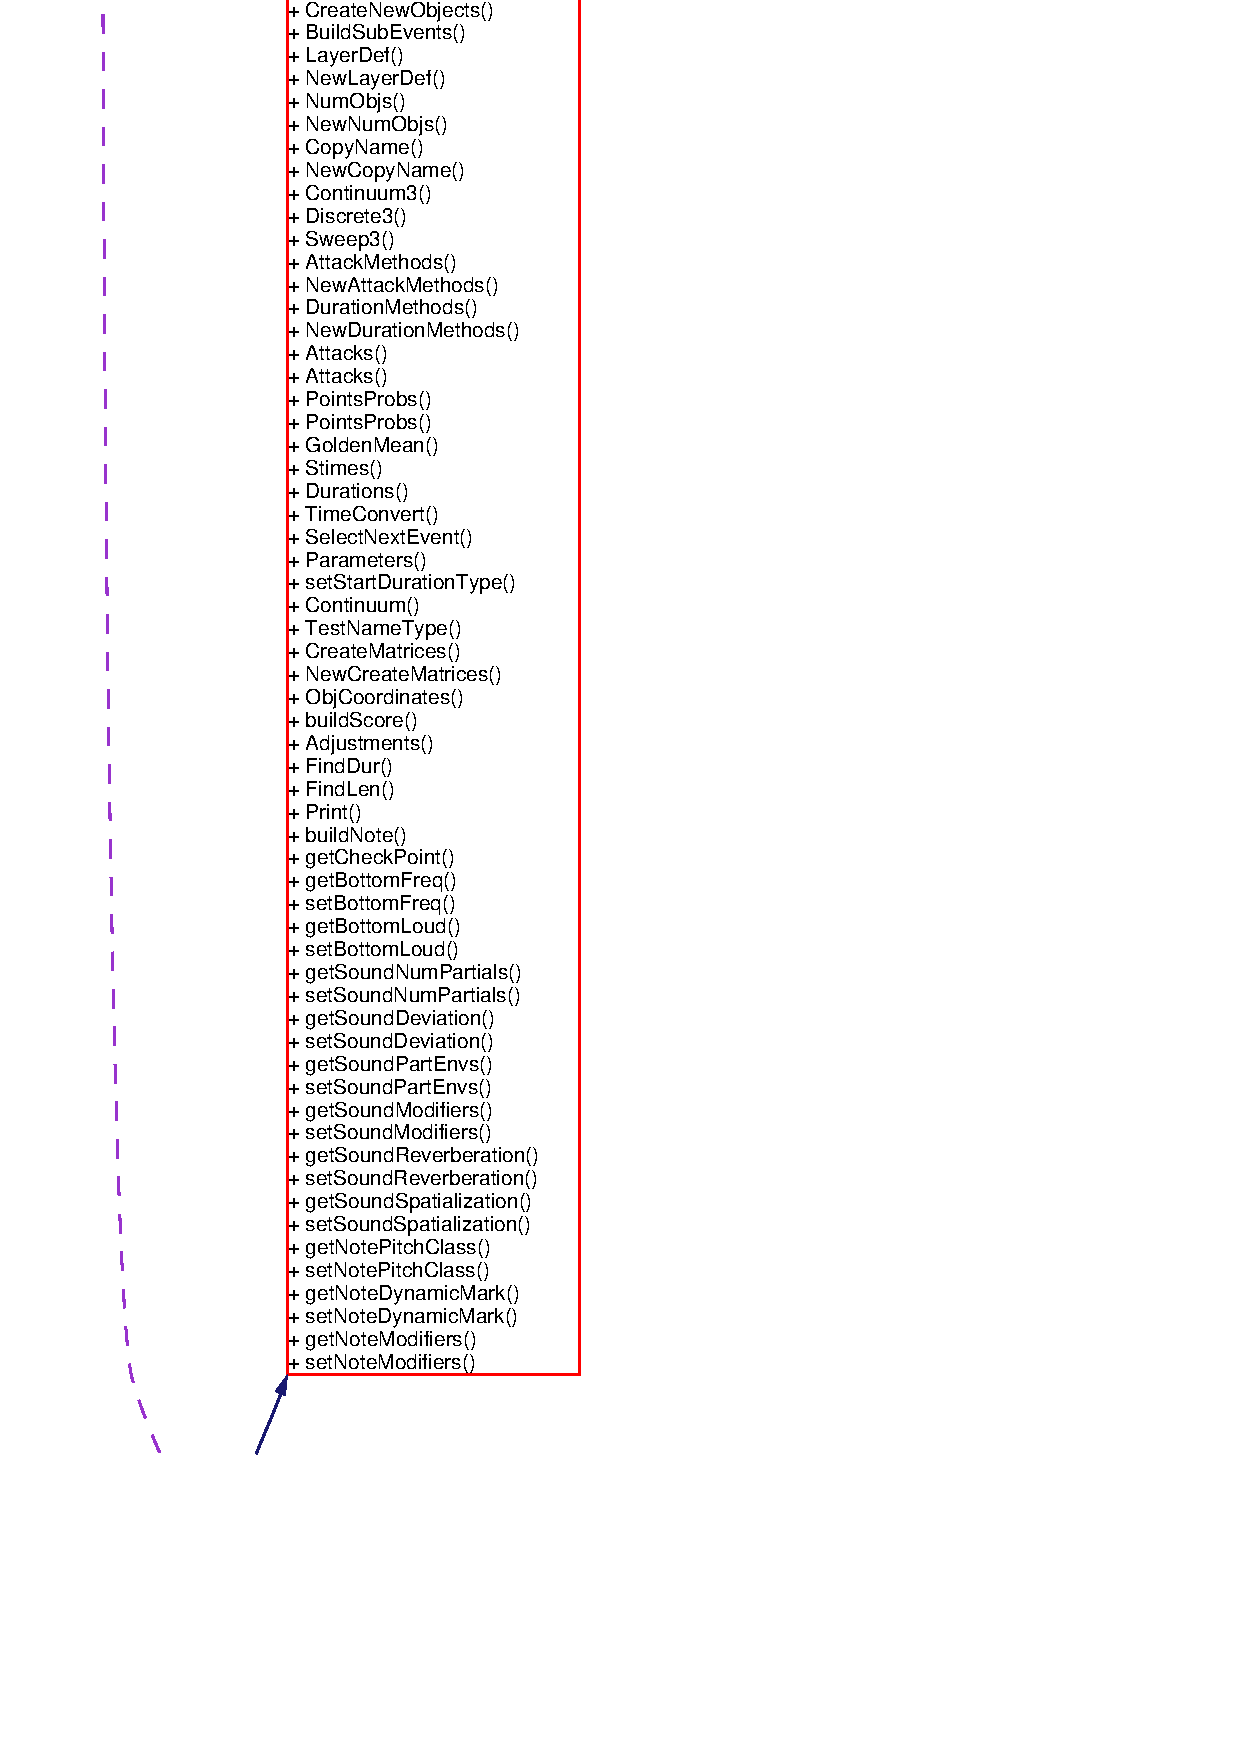
\includegraphics[width=139pt]{classLow__coll__graph}
\end{center}
\end{figure}
\subsection*{Public Member Functions}
\begin{CompactItemize}
\item 
{\bf Low} (float a\-Start\-Time, float a\-Duration, int a\-Type, char $\ast${\bf a\-Name})
\item 
{\bf Low} (const  {\bf Low} \&orig\-Low)
\item 
{\bf $\sim$Low} ()
\item 
{\bf Low} \& {\bf operator=} (const  {\bf Low} \&orig\-Low)
\item 
void {\bf clear} ()
\item 
void {\bf Print} ()
\end{CompactItemize}
\subsection*{Protected Attributes}
\begin{CompactItemize}
\item 
double {\bf low\-Density}
\end{CompactItemize}


\subsection{Constructor \& Destructor Documentation}
\index{Low@{Low}!Low@{Low}}
\index{Low@{Low}!Low@{Low}}
\subsubsection{\setlength{\rightskip}{0pt plus 5cm}Low::Low (float {\em a\-Start\-Time}, float {\em a\-Duration}, int {\em a\-Type}, char $\ast$ {\em a\-Name})}\label{classLow_a0}




Definition at line 47 of file low.cpp.

References Event::a\-Name, bottom\-ID, low\-ID, Event::set\-Density(), Event::set\-Duration(), Event::set\-Name(), Event::set\-Start\-Time(), and Event::set\-Type().

Here is the call graph for this function:\begin{figure}[H]
\begin{center}
\leavevmode
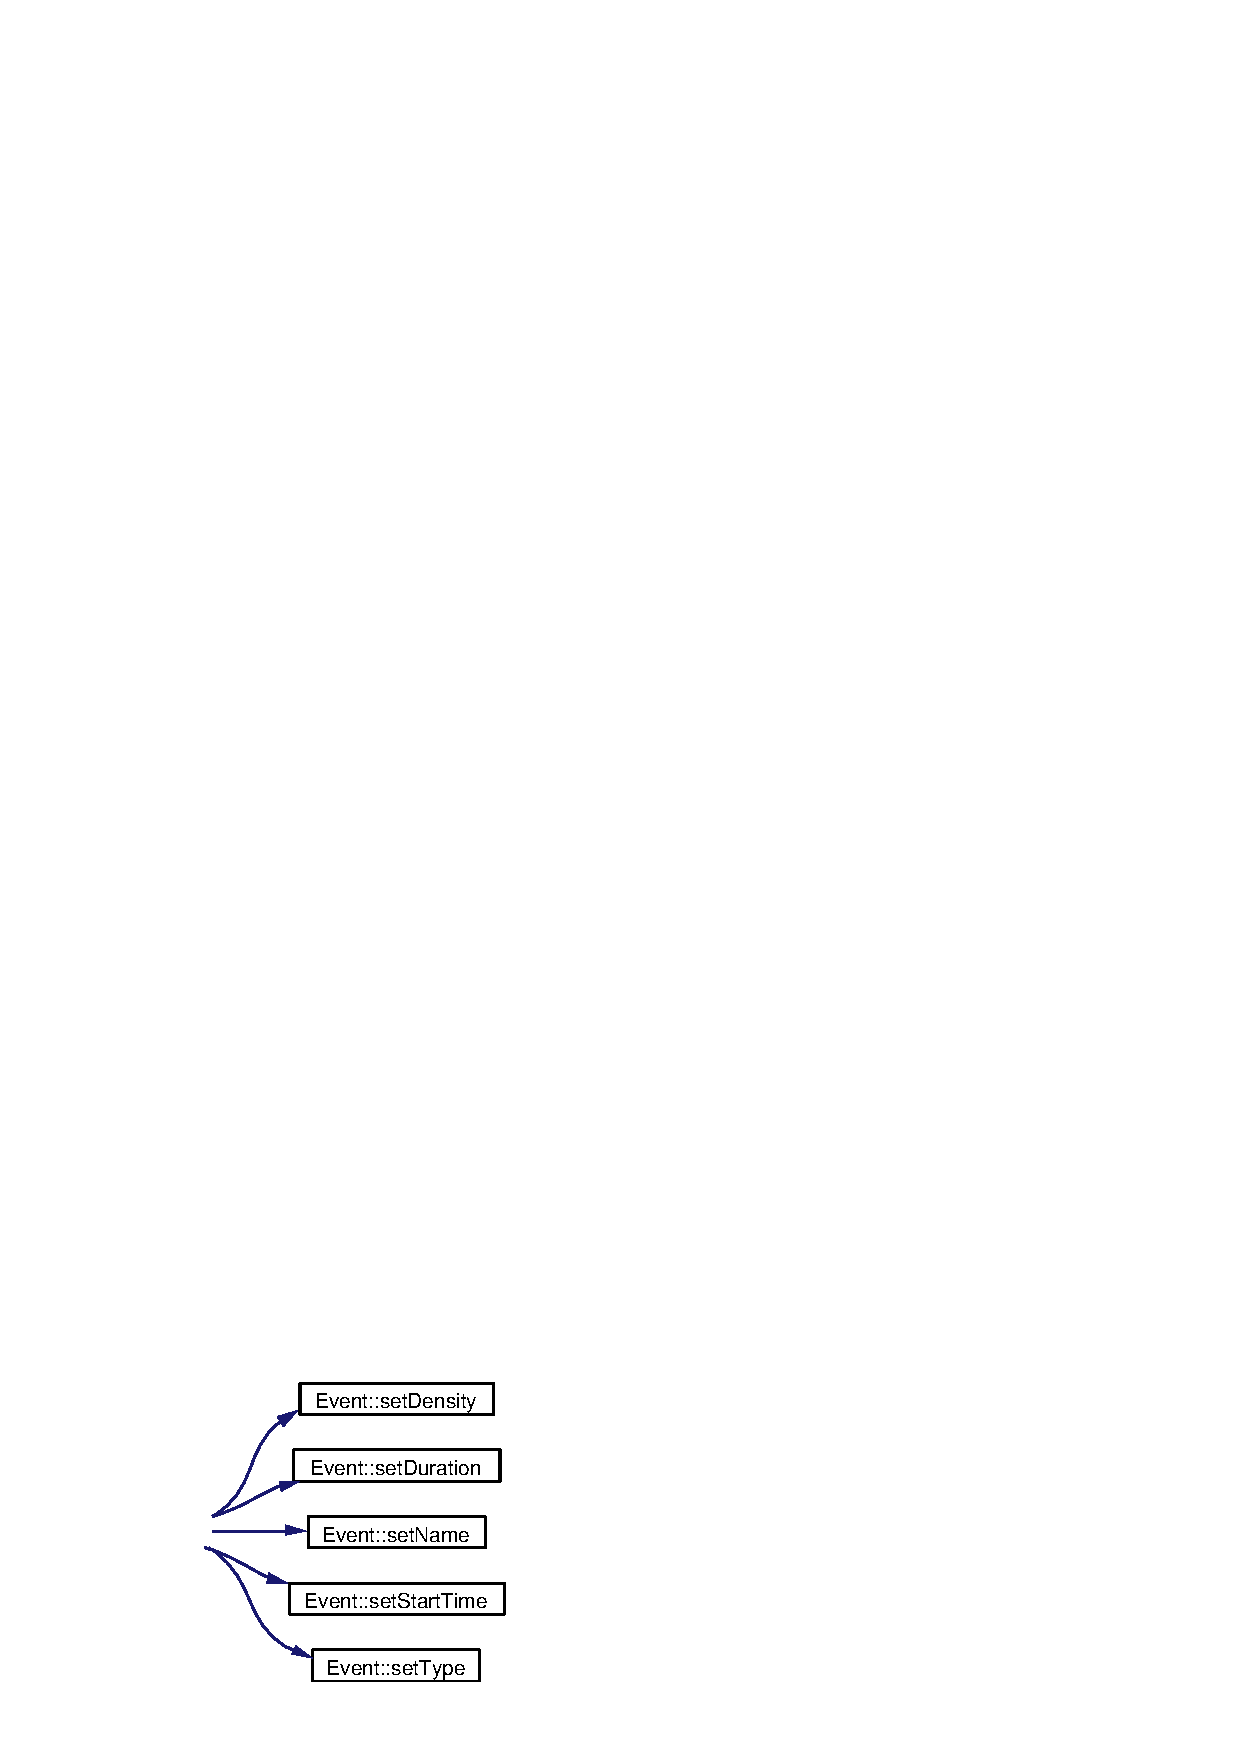
\includegraphics[width=125pt]{classLow_a0_cgraph}
\end{center}
\end{figure}
\index{Low@{Low}!Low@{Low}}
\index{Low@{Low}!Low@{Low}}
\subsubsection{\setlength{\rightskip}{0pt plus 5cm}Low::Low (const {\bf Low} \& {\em orig\-Low})}\label{classLow_a1}




Definition at line 79 of file low.cpp.

References bottom\-ID, and low\-ID.\index{Low@{Low}!~Low@{$\sim$Low}}
\index{~Low@{$\sim$Low}!Low@{Low}}
\subsubsection{\setlength{\rightskip}{0pt plus 5cm}Low::$\sim${\bf Low} ()}\label{classLow_a2}




Definition at line 91 of file low.cpp.

\subsection{Member Function Documentation}
\index{Low@{Low}!clear@{clear}}
\index{clear@{clear}!Low@{Low}}
\subsubsection{\setlength{\rightskip}{0pt plus 5cm}void Low::clear ()\hspace{0.3cm}{\tt  [virtual]}}\label{classLow_a4}


Clears several internal structures in the {\bf Event}{\rm (p.\,\pageref{classEvent})}: name\-Type, max\-Types, layer\-Dens, objs\-In\-Layer, remain\-Objs, types\-In\-Layer, star\-Tarray, prob\-Sieve\-Array, dur\-Array, prob\-Dur\-Array 

Reimplemented from {\bf Event} {\rm (p.\,\pageref{classEvent_a12})}.

Definition at line 100 of file low.cpp.\index{Low@{Low}!operator=@{operator=}}
\index{operator=@{operator=}!Low@{Low}}
\subsubsection{\setlength{\rightskip}{0pt plus 5cm}{\bf Low}\& Low::operator= (const {\bf Low} \& {\em orig\-Low})}\label{classLow_a3}


\index{Low@{Low}!Print@{Print}}
\index{Print@{Print}!Low@{Low}}
\subsubsection{\setlength{\rightskip}{0pt plus 5cm}void Low::Print ()\hspace{0.3cm}{\tt  [virtual]}}\label{classLow_a5}




Reimplemented from {\bf Event} {\rm (p.\,\pageref{classEvent_a57})}.

Definition at line 109 of file low.cpp.

References low\-ID, output\-File, Event::the\-Duration, Event::the\-Name, Event::the\-Start\-Time, and Event::u\-Per\-Sec.

\subsection{Member Data Documentation}
\index{Low@{Low}!lowDensity@{lowDensity}}
\index{lowDensity@{lowDensity}!Low@{Low}}
\subsubsection{\setlength{\rightskip}{0pt plus 5cm}double {\bf Low::low\-Density}\hspace{0.3cm}{\tt  [protected]}}\label{classLow_p0}




Definition at line 37 of file low.h.

The documentation for this class was generated from the following files:\begin{CompactItemize}
\item 
{\bf low.h}\item 
{\bf low.cpp}\end{CompactItemize}
